\documentclass[11pt]{article}
\usepackage[utf8]{inputenc}
\usepackage{mathtools}
\usepackage{vmargin}
\usepackage{graphicx}
\usepackage{lmodern}
\usepackage[T1]{fontenc}
\usepackage{multirow}
\usepackage[noline,ruled,linesnumbered,spanish]{algorithm2e}
\usepackage{forest}
\usepackage{forest,adjustbox}
\usepackage{color}

\setpapersize{A4}
\setmargins{2.5cm}       % margen izquierdo
{0cm}                        % margen superior
{16.5cm}                      % anchura del texto
{23.42cm}                    % altura del texto
{10pt}                           % altura de los encabezados
{1cm}                           % espacio entre el texto y los encabezados
{0pt}                             % altura del pie de página
{2cm}                           % espacio entre el texto y el pie de página

\title{Mini-Proyecto III: Estructuras de Datos Sucintas}
\author{Cristobal Donoso Oliva}
\author{
Diego Seco$^{1}$, Meraioth Ulloa Salazar$^{2}$, Cristóbal Donoso Oliva$^{3}$,\\ Matías Medina Silva$^{4}$,\\ \\
\small{$^{1}$Docente a cargo de la asignatura$^{2-3-4}$Estudiantes Pre-grado}\\
\small{$^{1-2}$Dpto. de Ingeniería Civil Informática y Ciencias de la Computación}\\
\small{Universidad de Concepción, Concepción, Chile.}\\
}
\date{Noviembre de 2016}
\usepackage{amsmath}
\begin{document}

\maketitle

\section{Range Minimum Query}
\subsection{Descripción del Problema}
El problema de RMQ (Range Minimum Query) consiste en encontrar el mínimo dentro de un rango [i,j] perteneciente a un arreglo de n objetos que se pueden comparar. En particular, resolveremos el problema para un arreglo de números. Usualmente debemos resolver RMQ en el desarrollo de otros problemas, tales como: Lowest Common Ancestors o del áres de Document Retrieval.
\begin{center}\begin{tabular}{|c|c|c|c|c|c|c|}
\hline
	13 & 2 & 7 & 0 & 9 & 10 & 27 \\
\hline
\end{tabular}
\\\scriptsize{\color{white}.\color{black}\\Figura 1: Data set con números}
\end{center}
Sea $RMQ$ la función que retorna el minimo del rango $[i,j]$, con 0$\le$i$\le$ j$\le$n, entonces: \begin{center}$RMQ[2,6] = 0$\\$RMQ[0,2] = 2$\\$RMQ[4,4] = 9$\end{center}  
En la práctica existen varias soluciones candidatas a este problema, sin embargo, no todas ellas rinden de igual manera. Con el objetivo de comparar experimentalmente la complejidad asociada al RMQ, \emph{utilizaremos dos implementaciones básicas y una estructura de datos sucinta}.

\subsection{Solución Naive}
Consiste en almacenar los mínimos asociados a todas las sub-cadenas que pertenecen al arreglo de números; con esto realizamos consultas en tiempo $O(1)$, sin embargo, la complejidad espacial asciende a $O(n^2)$. Cabe mencionar que en situaciones donde \emph{el recurso espacial no es relevante}, implementar esta solución es una alternativa rápida y sencilla a la hora de computar las consultas, sin embargo, es importante añadir que los datos consultados deben cumplir la condición de \emph{ser estáticos}, en su defecto, el dinamismo actualizaría la tabla frecuentemente aumentando el tiempo de pre-procesamiento.\\\\A continuación se muestra la matriz resultante del set de números propuesto anteriormente(ver figura 1).
\begin{center}$\begin{vmatrix}
	13 & 2 & 2 & 0 & 0 & 0 & 0 \\
	 & 2 & 2 & 0 & 0 & 0 & 0 \\
	 &  & 7 & 0 & 0 & 0 & 0 \\
	 &  &  & 0 & 0 & 0 & 0 \\
	 &  &  &  & 9 & 9 & 9 \\
	 &  &  &  &  & 10 & 27 \\
	 &  &  &  &  &  & 27 \\
\end{vmatrix}$
\\\scriptsize{\color{white}.\color{black}\\Figura 2: Matriz que guarda los mínimos parciales de todos los rangos de un conjunto de números}
\end{center}
Una consulta simple bastaría con preguntar por la dirección $<i,j>$ de la matriz generada.

\subsection{Solución RMQ + Sparse Table}
Podemos resolver el problema RMQ optimizando la matriz que almacena los mínimos utilizando potencias de dos para definir la dimensión de la tabla (sparse table). Esta alternativa nos permite disminuir el espacio realizando consultas en tiempo constante. En efecto, las complejidades asociadas al espacio y consulta son $O(nlog(n))$ y $O(1)$ respectivamente.\\\\La cantidad de filas corresponden a los datos en el set, sin embargo, las columnas responden a $O(log(n))$. La idea consiste en pre-computar el mínimo de todas las sub-cadenas de tamaño $2^k$ donde $0 \le k \le log(n)$. Del mismo set (figura 1) la tabla generada es:

\begin{center}$\begin{vmatrix}
	0 & 1 & 3   \\
	1 & 1 & 3   \\
	2 & 3 & 3   \\
	3 & 3 &     \\
	4 & 4 &     \\
	5 & 5 &     \\
	6 &   &	    \\
\end{vmatrix}$
\\\scriptsize{\color{white}.\color{black}\\Figura 2: Sparse Table para el set}
\end{center}
Para calcular la tabla es necesario saber la cantidad de columnas $j$ que tendrá la tabla, para ello calculamos:
\begin{center}$\#j$ = log(\emph{$\#$ elementos})  $\iff \lfloor log(7) \rfloor+1 \iff 2 +1 = 3$
\end{center}
Donde $\#$ representa la cardinalidad y $log$ es de base 2. Luego buscamos los mínimos que se encuentran dentro de los rangos $2^j$ con $0\le j \le 2$ para cada posición $i$. Para realizar la consulta debemos comparar:
\begin{center}$arr[lookup[i][j-1]]$ $\nabla$ $arr[lookup[i+2^j-1-1][j-1]]$\end{center}
Donde $\nabla$ = $\{\le,\geq\}$. RMQ retorna el menor entre los valores comparados. 

\subsection{Solución RMQ Succinct}
RMQ Succinct es, teóricamente, la mejor alternativa a la hora de computar las busquedas de un mínimo dentro de un set. Esta solución utiliza la técnica de Indirección con el objetivo de simplificar aún más la complejidad asociada al espacio.\\\\La idea consiste en generar $\frac{2n}{log(n)}$ bloques de tamaño $\frac{1}{2}log(n)$ e ir guardando resúmenes en cada nivel de manera que acceder a los datos mínimos sea muy rápido.  
\begin{figure}[htp]
\centering
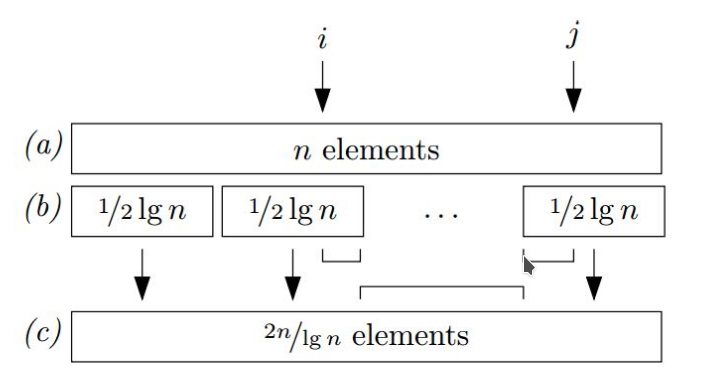
\includegraphics[scale=0.5]{indirecion.png}
\\\scriptsize{\color{white}.\color{black}\\Figura 3: Representación gráfica de los bloques generados en un modelo de indirección}
\label{}
\end{figure}
Con todo esto logramos obtener espacio $O(n)$ y $O(1)$ consulta.\\\\En la práctica utilizaremos la librería SDSL (https://github.com/simongog/sdsl-lite) la cual trae implementado un RMQ sucinto. Haremos uso de del método \textbf{rmq} de la clase \emph{rmq\_succinct\_sct} al cual le pasamos como parámetros los límites del rango a considerar.
\subsection{Experimento y Resultados}
Anteriormente determinamos teóricamente la complejidad espacial de los tres algoritmos en cuestión. Es fácil demostrar en la práctica como influye la construcción de las tablas ya que éstas alteran la tiempo de ejecución en directa proporción con la cantidad de elementos. En ese sentido, al realizar consultas bajo \emph{datasets} espacialmente dinámicos, las soluciones deberían diferir bastante entre sí.\begin{center}\emph{\textbf{Hipótesis}\\Para un vector de tamaño variable y que almcaena número la alternativa Sucinta saca ventaja en tiempo a los otras alternativas.}\end{center}Para realizar los experimentos se utilizó un procesador \emph{AMD Phenom(tm) 9550 Quad-Core Processor} y se dispuso de 8GB de RAM. \\\\Para los \emph{sets aleatorios} de tamaño $10^i$ con 0<i<$10^7$ y rango $[0,random(0...i)]$ se obtuvieron los siguientes resultados:
\begin{center}\begin{tabular}{|l|c|c|c|}
\hline
	$Tamaño$ & $Naive$ & $Sparse$ & $Succinct$\\
\hline
	10       & 7.7e-5   & 4.4e-5      & 2.4e-05\\
\hline
	100 	 & 0.002429 & 0.000441    & 4.7e-05 \\
\hline
	1000     & 0.097398 & 0.004381    & 0.000217\\
\hline
	10000    & 8.8443   & 0.031585    & 0.00169\\
\hline
	100000   & killed   & 0.0323302   & 0.003774\\
\hline
	1000000  & killed   & 3.63675     & 0.034628\\
\hline
	10000000 & killed   & 40.3935     & 0.349027\\
\hline
\end{tabular}
\\\scriptsize{\color{white}.\color{black}\\Figura 4: Tabla de resultados tiempo de ejecución algoritmos propuestos}
\end{center}
Para mayor claridad solo se muestra el gráfico hasta i = 800 puesto que las rectas difieren mucho producto del orden de complejidad.
\begin{center}\begin{figure}[htp]
\centering
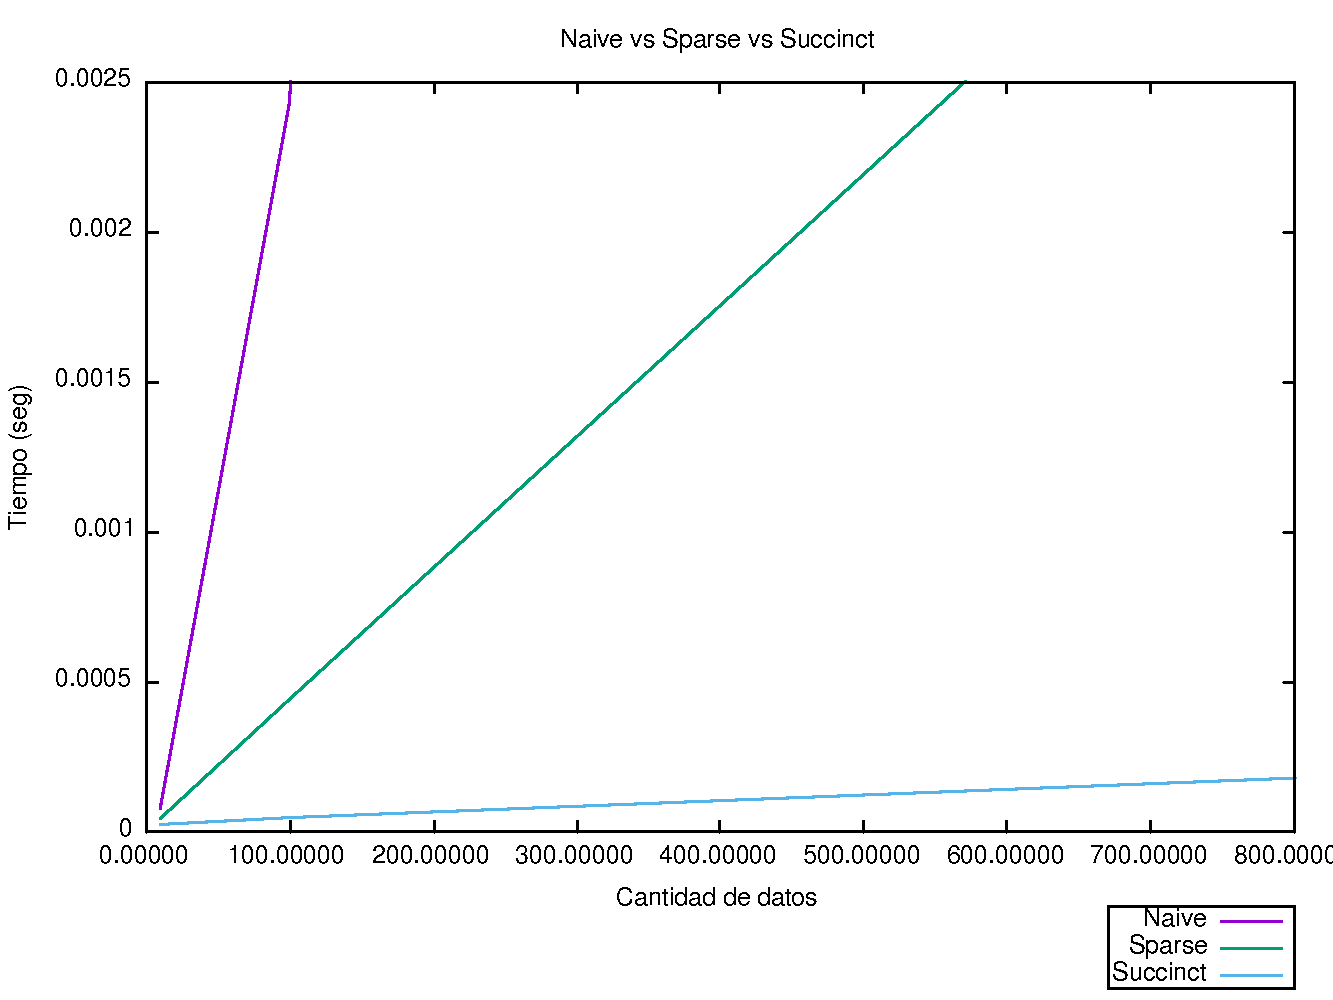
\includegraphics[scale=0.6]{grafico.pdf}
\\\scriptsize{\color{white}.\color{black}\\Figura 5: Bifurcación que muestra las diferencias en tiempo de ejecución de los algoritmos naive y sparse}
\label{etiqueta}
\end{figure}
\end{center}
Se puede apreciar como la alternativa sucinta saca ventaja de su compresión. A raíz de los resultados empíricos es posible reconocer cuales son las mejores alternativas. En el caso particular de la solución Naive, vemos como se dispara de manera cuadrática la curva. En escenarios donde no importa el recurso memoria naive se podría utilizar, sin embargo, la mayoría de los problemas actuales necesitan manejo de grandes volúmenes de datos. Sparse significa una simplificación importante y podría ser útil para volúmenes de hasta $10^5$ datos, consideramos más fácil de implementar que una estructura de datos sucinta.Aún cuando los recursos sean abundantes y la dificultad del código no sea problema, tratamos de buscar la alternativa más rápida y de menor espacio (considerando que todos los recursos son escasos y debemos optimizarlos).
\end{document}
